\documentclass[a4paper]{article}

\usepackage{fullpage} % Package to use full page
\usepackage{parskip} % Package to tweak paragraph skipping
\usepackage{tikz} % Package for drawing
\usepackage{amsmath}
\usepackage{hyperref}
\usepackage{enumitem}
\usepackage{booktabs}
\usepackage{listings}
\title{Homework }
\author{Jeff Tilton}
\date{September, 30 2019}
\usepackage{graphicx}
\usepackage{subcaption}
\begin{document}

\maketitle

\section{K-means}
\textit{Note:} kmeans.py has code related to this problem.

Given m = 5 data points configuration in Figure 1. Assume K = 2 and use Euclidean distance. Assuming the initialization of centroid as shown, after one iteration of k-means algorithm, answer the following questions.

\begin{enumerate}[label=(\alph*)]
\item Show the cluster assignment
\item Show the location of the new center
\item Will it terminate in one step?
\end{enumerate}

\subsection{Steps for K-means}

I went through the below steps to complete the questions for k-menas for both Euclidean and Manhattan norms.

\begin{enumerate}
\item Assign points to closest cluster center using specified norm as distance metric.
\item Average points within each cluster.
\item Assign new cluster centers based on the answer from step 2.
\end{enumerate}



\subsection{Euclidean Distance}


\begin{align}
d(\mathbf{p},\mathbf{q}) = d(\mathbf{q},\mathbf{p}) & = \sqrt{(q_1-p_1)^2 + (q_2-p_2)^2 + \cdots + (q_n-p_n)^2} 
& = \sqrt{\sum_{i=1}^n (q_i-p_i)^2}
\end{align}

\begin{enumerate}[label=(\alph*)]
\item The Cluster assignment after the first iteration is $(1,3), (2,4,5)$
\item New cluster centers are seen in figure 1 below.
\item K-means does not terminate after one step.  Centers after one step are: $(-1.5, -0.5), (1.67, 0.67)$.  After convergence: $(-1.0, -0.67), (2.5, 1.5)$
\end{enumerate}

\begin{figure}[h]	
	\centering
		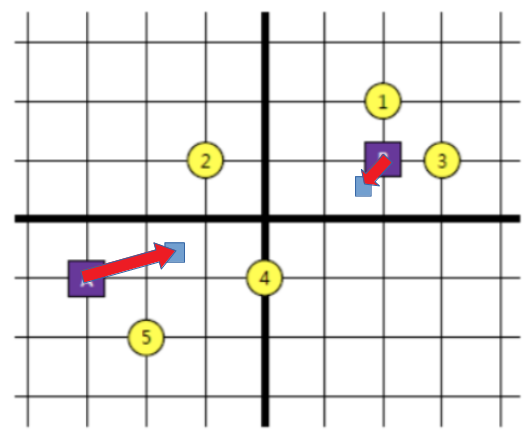
\includegraphics[width=5cm, height=5cm]{Q1_euclidean.png}
		\caption{New cluster centers after one iteration of K-means using Euclidean distance}
\end{figure}


\newpage
\subsection{Manhattan Distance}


$$d_1(\mathbf{p}, \mathbf{q}) = \|\mathbf{p} - \mathbf{q}\|_1 = \sum_{i=1}^n |p_i-q_i|$$


\begin{enumerate}[label=(\alph*)]
\item The Cluster assignment after the first iteration is $(1,3), (2,4,5)$
\item New cluster centers are seen in figure 2 below.
\item K-means terminates after one step.  Centers after one step are: $(-1.0, -0.67), (2.5, 1.5)$.  After convergence: $(-1.0, -0.67), (2.5, 1.5)$.
\end{enumerate}

\begin{figure}[h]
	\centering
		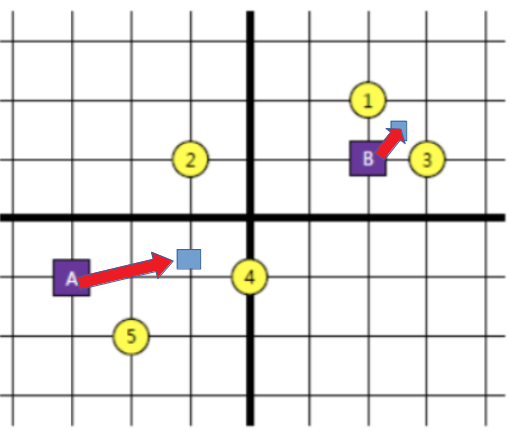
\includegraphics[width=5cm, height=5cm]{Q1_manhattan.png}
		\caption{New cluster centers after one iteration of K-means using Manhattan distance}
\end{figure}


It is interesting to note the difference between the 2 measures.  Point 4 is assigned to cluster B in the Euclidean distance and pulls the cluster center towards it for the first iteration.  It then is reassigned to cluster A.  Point 4 is assigned to cluster A immediately using the Manhattan distance.  This is the reason that K-means is able to terminate after one iteration using the Manhattan distance, but multiple iterations are needed for the Euclidean distance.

\section{Spectral Clustering}
\textit{Note:} spectral.py has all code related to this question.

Spectral clustering goes beyond K-means, which only considers distance, and also takes the data geometry into account.  Spectral clustering uses an adjacency matrix to capture the connectedness between the data points to cluster data.  The data was clustered into 2 clusters in figure 3 below using k-nearest neighbors to create an adjacency matrix. A good way to think about this is that points are similar to each other if they can reach each other by small jumps through the data cloud.

Although nodes $(0, 0)$ and $(-1, 0)$ are closest to each other, they are in separate clusters because of the geometry of the data.  Using only K-means provided a much different result.


\begin{figure}[h]
    \centering
    \begin{subfigure}[b]{0.3\textwidth}
        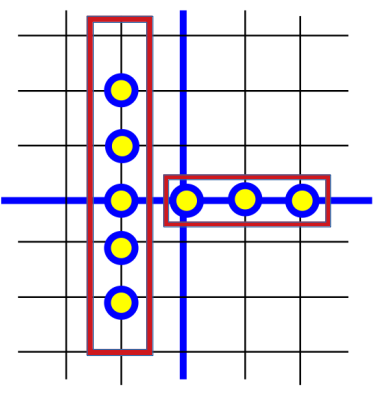
\includegraphics[width=\textwidth]{Q2_spectral.png}
        \caption{Cluster results from spectral clustering.}
        \label{spectral}
    \end{subfigure}
    \begin{subfigure}[b]{0.3\textwidth}
        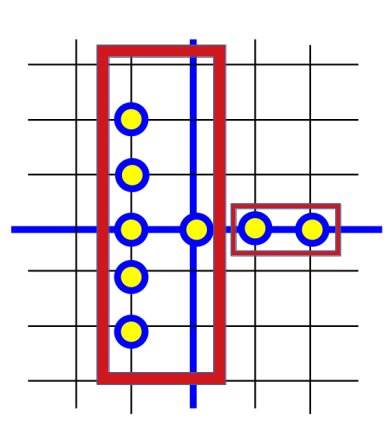
\includegraphics[width=\textwidth]{Q2_kmeans.png}
        \caption{Cluster results using K-means clustering.}
        \label{kmeans}
    \end{subfigure}

    \caption{Two different clustering algorithm results on the same dataset.  The spectral clustering used k nearest neighbors with 2 neighbors to build an adjacency matrix, then k-means on the results from eigendecomposition on the Laplacian matrix.  K-means used Euclidean distance as measure. }\label{clusterCompare}
\end{figure}



\section{Principal Component Analysis}
\textit{Note:} pc.py contains all code for this section.

Suppose we have 4 points in 3-dimensional Euclidean space, namely $(4, −2, 4), (5, −3, 5),
(2, 0, 2),$ and $(3, −1, 3).$

\subsection{Find the first principal direction.}

The first principal direction is the eigenvector associated with the highest eigenvector.  THe steps listed below are how to find the $n$ principal directions of a dataset.

\begin{enumerate}
\item Standardize the data, although I found conflicting information online, a post from  Mohammad Mohammadpour Salut (@388) said to standardize the data to have a zero mean and unit variance.
\item Create the square covariance matrix.
\item Perform eigendecomposition on the covariance matrix.
\item Order the eigenvectors in descending order of their associated eigenvalues.
\item Choose the first $n$ eigenvectors as your principal components/directions.
\end{enumerate}

After performing these steps on the given data I calculated the first principal direction below. 

$$[ 0.57735027, -0.57735027,  0.57735027]$$.

\subsection{When we reduce the dimensionality from 3 to 1 based on the principal direction you found above, what is the reconstruction error in terms of variance?}

PCA can be thought of in 2 ways.  First, as maximizing the variance of your first $j$ components.  Or, secondly, minimizing the last $j$ components.  Eigenvalues represent the variance explained by a component, therefore the reconstruction error in terms of variance is the sum of the last 2 eigenvalues, which equals 3.02.





\subsection{You are given the following 2-D datasets, approximately draw the first and second
principal directional on each plot.}


Optimization for PCA either maximizes the variance or minimizes the reconstruction error.  Looking at the images below, it is easy to see the first principal direction in plot a.  The variance is greatest as a negative slope, which would minimize reconstruction, much like least squares regression.  The second plot is a little harder to tell, but the first 2 principal directions form a cross with the first principal direction aligned in the vertical direction.

 

\begin{figure}[h]
    \centering
		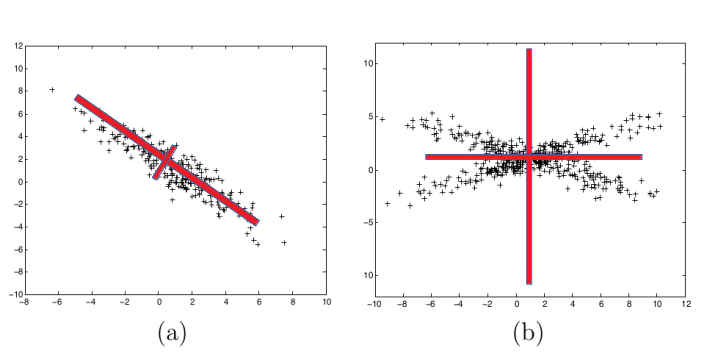
\includegraphics[width=\textwidth]{pca_clouds.png}
        \caption{The first 2 principal directions of 2 data clouds.}
\end{figure}


\newpage
\section{Eigenfaces}

\textit{Note:} eigen.py contains all code for this section.

\subsection{Produce eigenfaces for given dataset}

I followed the steps below to produce the eigenfaces.

\begin{enumerate}
\item Downsampled the data using the skimage library to shape $(m,n)$.
\item Vectorized the images.
\item Standardize the data, although I found conflicting information online, a post from  Mohammad Mohammadpour Salut (@388) said to standardize the data to have a zero mean and unit variance.
\item Create the square covariance matrix.
\item Perform eigendecomposition on the covariance matrix.
\item Order the eigenvectors in descending order of their associated eigenvalues.
\item Choose the first $n$ eigenvectors as your principal components/directions.
\item Projected the data from centered data for first 6 eigenvectors.
\end{enumerate}

\subsubsection{Plot the top 6 eigenfaces for each subject}
eigenfaces.py produced the figure below.

\begin{figure}[h]
	\centering
		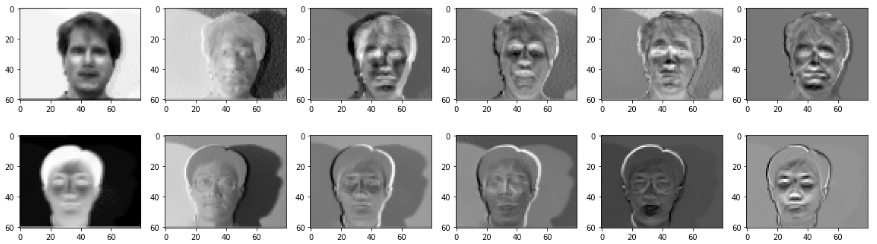
\includegraphics[ height=4cm]{eigenfaces.png}
		\caption{Eigenfaces produced with the first 6 eigenvectors of 2 different face subjects.}
\end{figure}

\subsubsection{What is the interpretation of the top 6 eigenfaces?}

The top eigenvectors are the maximum variation in a face and can be interpreted as the most prominent features.   

\subsection{Face Recognition}

I used the numpy library to calculate te Pearson correlation coefficient (below) to use as a score for the eigenfaces and test photo.

$$\rho = \frac{\text{cov}(X,Y)}{\sigma_x \sigma_y}$$

\begin{table}[ht]
\centering
\caption{Mean correlation coefficients between test photo and eigenfaces 1-6}
\begin{tabular}[t]{lcc}
\toprule
&Test photo 01&Test photo 14\\
\midrule
Subject 01&0.17&0.003\\
Subject 14&0.05&-0.15\\
\bottomrule
\end{tabular}
\end{table}%


Table one shows that you can use eigenfaces for face recognition by taking the largest absolute value of the correlation coefficient.  The mean value between the eigenfaces from subject 01 and the test face 01 has an absolute value of 0.17 compared to the mean correlation coefficient of test face 14 of 0.003.  Likewise the mean value between the eigenfaces of subject 14 and the test face 14 has an absolute value of 0.15 compared to the mean value of test face 01 of 0.05.

\section{ISOMAP}
\textit{Note:} isomap.py contains all code for this section.


\subsection{Visualize the similarity graph (e.g., plot the adjacency matrix where weights are shown using intensity).}

I created the similarity graph with vertices corresponding to the images, and connecting each image to the $k$ nearest neighbors in the dataset, for $k = 100$ in the file isomap.py.  I also made a weight graph with the vertices corresponding to the euclidean distance for the $k$ nearset neighbors or an arbitrarily long distance for all other values. 

\begin{figure}[h]
    \centering
    \begin{subfigure}[b]{0.3\textwidth}
        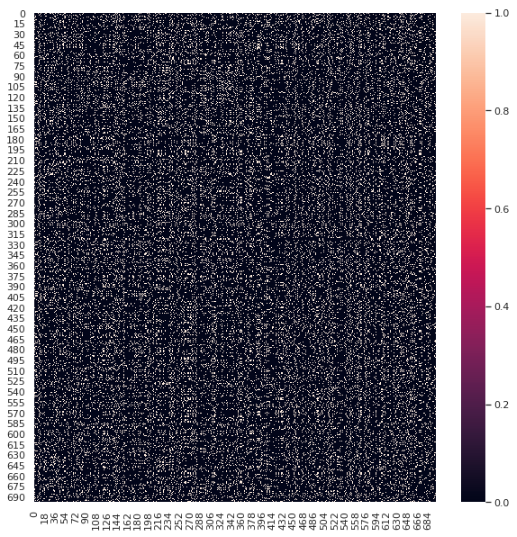
\includegraphics[width=\textwidth]{a.png}
        \caption{A}
        \label{A}
    \end{subfigure}
    \begin{subfigure}[b]{0.3\textwidth}
        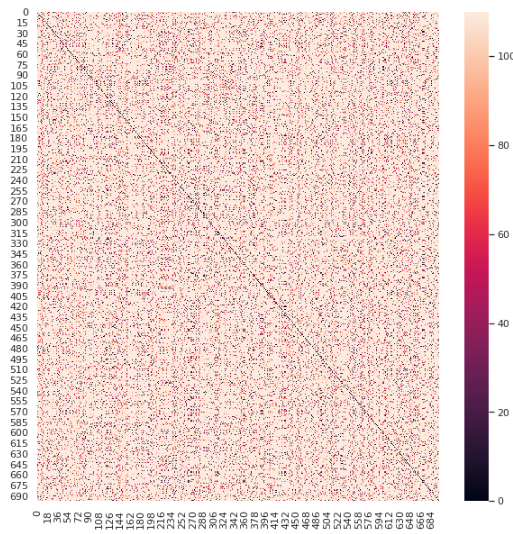
\includegraphics[width=\textwidth]{w.png}
        \caption{W}
        \label{W}
    \end{subfigure}
    \caption{Two similarity Graphs. A: Similarity graph with vertices corresponding to a 1 for the first $k=100$ nearest neighbors, 0 otherwise. W: Similarity graph with vertices corresponding to the euclidean distance for the first $k=100$ nearest neighbors, arbitrarily large value otherwise.}\label{clusterCompare}
\end{figure}

\subsection{Implement the ISOMAP algorithm and apply it to this graph to obtain a d = 2-dimensional embedding. Present a plot of this embedding. Find three points that are close to each other and show what they look like. Do you see any similarity among them?}


I implimented the Isomap algorithm in python as seen below.
\newpage
\begin{lstlisting}[language=Python]
impoert pandas as pd
import numpy as np
from scipy.spatial.distance import cdist
import networkx as nx

def Matrix_D(W):
    n = np.shape(W)[0]
    Graph = nx.DiGraph()
    for i in range(n):
        for j in range(n):
            Graph.add_weighted_edges_from([(i,j,min(W[i,j], W[j,i]))])

    res = nx.all_pairs_dijkstra_path_length(Graph)
    D = np.zeros([n,n])
    for i in range(n):
        for j in range(n):
            D[i,j] = res[i][j]
    np.savetxt('D.csv', D)
    return D

imgs = pd.read_csv('isomap.csv', header=None)
imgs.shape

X = imgs.values.T

dists = cdist(X, X, 'euclidean')

def get_w_matrix(a):
    idx = a.argsort().argsort()
    idx = np.array([x if x <= 100 else 110 for x in idx]).reshape(idx.shape)
    return idx

W = np.apply_along_axis(get_w_matrix, 1, dists)
D = Matrix_D(W)

m,_ = D.shape
I = np.identity(m)
ones = np.ones(D.shape)
H = I - (ones * 1/m)
C = np.dot(np.dot(H,D*D),H) * -1/(2*-10000000)
vals, vecs = np.linalg.eig(C)
pc_vals = vals[vals.argsort()[::-1]]
pcs = vecs[vals.argsort()[::-1]]

Zt = np.dot(pcs[:,:2],np.diag(pc_vals[:2]**(-.5)))
\end{lstlisting}

\newpage
\begin{figure}[h]
    \centering
    \begin{subfigure}[b]{0.4\textwidth}
        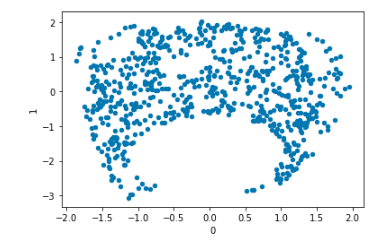
\includegraphics[width=\textwidth]{embedding.png}
        \caption{ISOMAP embedding}
        \label{embedding}
    \end{subfigure}
    \begin{subfigure}[b]{0.4\textwidth}
        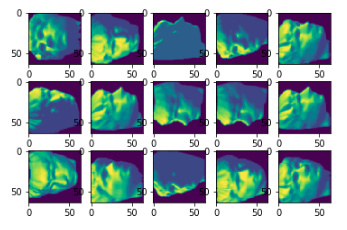
\includegraphics[width=\textwidth]{iso_faces.png}
        \caption{Close proximity faces}
        \label{iso_faces}
    \end{subfigure}
    \caption{Plot a shows the 2-dimensional embedding of the faces after the ISOMAP algorithm is applied.  Figure b is a selection of 3 groups of 5 faces that are in close proximity after ISOMAP dimensionality reduction.}\label{clusterCompare}
\end{figure}


The majority of the faces in each row face the same direction, but not all of them.  Four out of the five faces in the first row are facing a similar direction, 3 out of 5 in the 2nd row and 3 out of 5 in the 3rd.  

This is just taking the figures that are in close proximity to each other and not following any type of non-linear pattern.  I would have to use some labeled data and continue to test this algorithm before I felt confident deploying it.  If I had labeled data I could see how well it groups the data.  



\end{document}